\documentclass[12pt,a4paper]{article}
\usepackage[utf8]{inputenc}
\usepackage[french]{babel}
\usepackage[T1]{fontenc}
\usepackage{mathtools}
\usepackage{amsfonts}
\usepackage{amssymb}
\usepackage[pdftex]{graphicx}
\usepackage{comment}
\usepackage{siunitx}
\usepackage{csquotes}
\usepackage{caption}
\usepackage{tikz}
\usetikzlibrary{datavisualization}
\usetikzlibrary{babel}
\usepackage{pgfplots}
\pgfplotsset{compat=1.13 }
\usetikzlibrary{plotmarks}
\usepackage[colorinlistoftodos,prependcaption,textsize=tiny]{todonotes}
\usepackage[left=2cm,right=2cm,top=2cm,bottom=2cm]{geometry}
\author{Angelo Ortiz}
\title{Rapport du Projet Sorting Robot}
\graphicspath{ {../img/report/} }
% \renewcommand\thefootnote{\fnsymbol{footnote}}

\begin{document}
\begin{titlepage}
  \centering
  
\includegraphics[width=0.30\textwidth]{logo}\par\vspace{1cm}
  {\scshape\LARGE Sorbonne Universit\'e\par}
  \vspace{1cm}
  {\scshape\Large 2I006 : Algorithmique appliqu\'ee et structures de 
donn\'ees\par}
  \vspace{1.5cm}
  {\Large \bfseries Projet :\par}
  {\huge\bfseries Sorting Robot\par}
  \vspace{2cm}
  {\Large\itshape Kamil Rzeszutko\par}
  {\Large\itshape Angelo Ortiz\par}
  \vfill
  
  % Bottom of the page
  {\large Licence d'Informatique\par}
  {\large Ann\'ee 2017/2018\par}
\end{titlepage}
 
%\newpage
\tableofcontents
\listoffigures

\newpage
  
\part*{Introduction}
\section*{Pr\'esentation}
Le projet a consist\'e en la r\'esolution du probl\`eme du robot 
trieur au travers de diff\'erentes m\'ethodes.

Le jeu se compose d'une grille de jeu de $m$ lignes et $n$ colonnes et d'un 
robot pouvant se d\'eplacer sur la grille de jeu. Chaque case poss\`ede une 
couleur de fond et peut comporter une pi\`ece color\'ee. Le nombre de couleurs 
utilis\'ees dans la grille est $1 \leq c \leq m \cdot n$. Le but du jeu 
consiste \`a d\'eplacer le robot de sorte que chaque pi\`ece soit rang\'ee sur 
une case de m\^eme couleur. \`A chaque fois qu'une pi\`ece est amen\'ee sur une 
case de m\^eme couleur, la case devient noire. Le but est donc d'obtenir un 
\'ecran noir.

\section*{Objectif}
Le but de ce travail a \'et\'e de sensibiliser les étudiants sur l'impact des 
choix d'impl\'ementations, notamment au niveau des structures de données et 
leurs algorithmes plus adapt\'es, sur le temps d'ex\'ecution et l'espace 
m\'emoire r\'equis.

Dans le cadre du projet, on a utilis\'e les listes doublement cha\^in\'ees, les 
arbres AVL et les graphes orient\'es comme base des algorithmes mis en \oe uvre 
; on a aussi eu besoin d'une impl\'ementation de pile pour le dernier 
algorithme propos\'e.

\section*{Aper\c{c}u}
Il est possible de jouer au jeu du robot trieur \`a travers une interface 
graphique. Les d\'eplacements possibles sont associ\'es aux touches 
fl\`eches du clavier, et l'\'echange de pi\`eces se fait avec l'appui de 
la touche espace. On vous en pr\'esente un exemple dans la figure \ref{fig:gui}.

\begin{figure}[!h]
  \centering
  \captionsetup{justification=centering}
  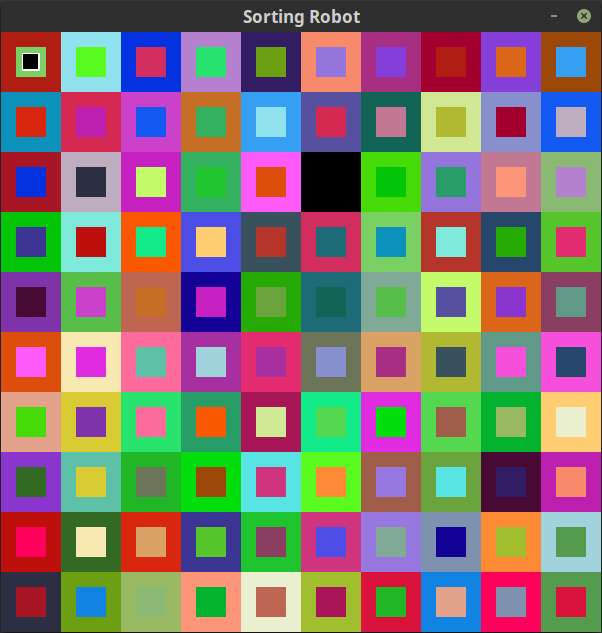
\includegraphics[width=0.5\textwidth]{gui}
  \caption[L'interface graphique du jeu]{L'interface graphique du jeu pour une 
  grille de 10x10 avec le robot dans la case en haut \`a gauche rep\'er\'e par 
un petit carr\'e noir avec une ligne blanche l'entourant}
  \label{fig:gui}
\end{figure}

Comme vous pouvez apercevoir dans le menu en console de la figure 
\ref{fig:console}, on a regroup\'e nos diff\'erents algorithmes de r\'esolution 
du probl\`eme donn\'e de sorte que l'on puisse trouver en m\^eme 
temps des diff\'erentes solutions pour une configuration du jeu donn\'ee.

\begin{figure}[!h]
  \centering
  \captionsetup{justification=centering}
  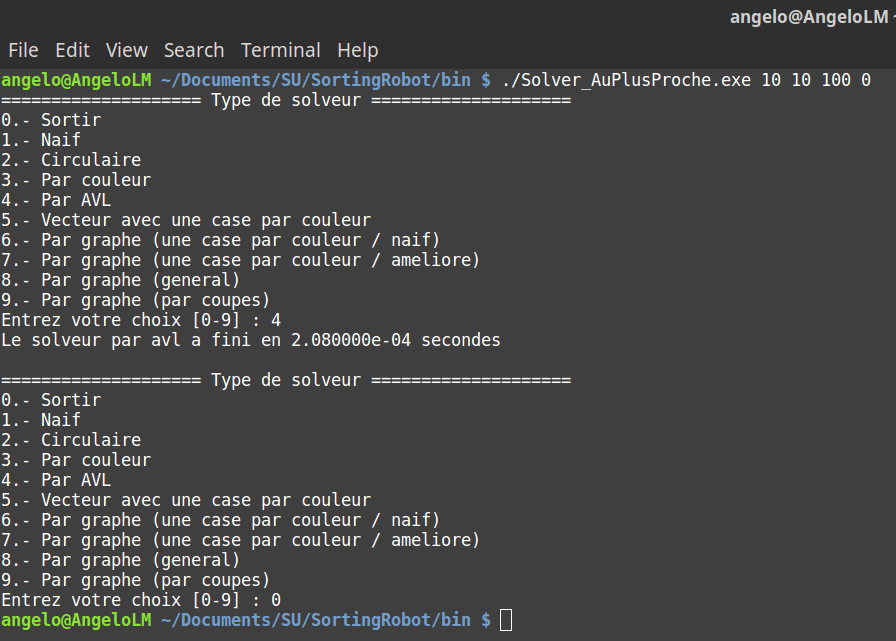
\includegraphics[width=0.9\textwidth]{console}
  \caption[Le menu en console]{Le menu en console permettant de 
	r\'esoudre le probl\`eme du robot \`a l'aide des 9 algorithmes 
impl\'ement\'es}
  \label{fig:console}
\end{figure}

\section*{Structure}
Le projet a \'et\'e organis\'e de mani\`ere coh\'erente en plusieurs 
r\'epertoires pour faciliter l'acc\`es aux morceaux de code recherch\'es.

\begin{figure}[!h]
  \centering
  \captionsetup{justification=centering}
  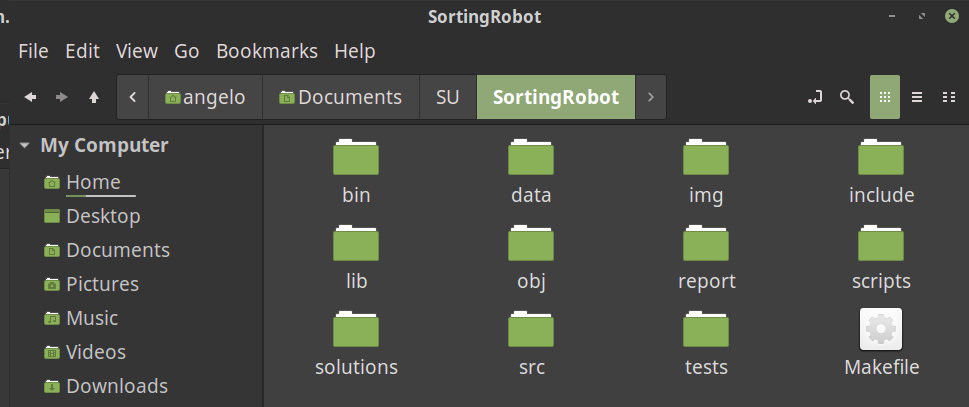
\includegraphics[width=0.9\textwidth]{structure}
  \caption[La structure projet]{La structure du projet en diff\'erents 
r\'epertoires et le fichier d'aide \`a la compilation \texttt{Makefile}}
  \label{fig:structure}
\end{figure}

Dans un premier temps, on se focalise sur le c\oe ur du projet, \`a 
savoir toute la partie li\'ee au code. Le r\'epertoire {\bfseries lib} contient 
les fichiers sources fournis aussi bien de la premi\`ere partie que de la 
deuxi\`eme partie. On a regroup\'e les fichiers sources des fonctions de base 
et des algorithmes de r\'esolution dans le r\'epertoire {\bfseries src}. Les 
fichiers d'en-t\^ete associ\'es aux fichiers sources de ces deux r\'epertoires 
se trouvent dans {\bfseries include}. Les fichiers de test de fonctionnement et 
performance, et d'exploitation des donn\'ees sont r\'epertori\'ees dans 
{\bfseries tests}. \`A l'issue de la compilation des fichiers \texttt{.c} du 
projet g\'er\'ee par {\bfseries Makefile}, on compte des fichiers objets et des 
ex\'ecutables : les premiers sont enregistr\'es dans {\bfseries obj} et les 
deuxi\`emes, dans {\bfseries bin}. 

Dans un deuxi\`eme temps, on d\'etaille la partie du projet d\'edi\'ee au 
traitement des donn\'ees obtenues. On compte notamment le r\'epertoire 
{\bfseries data} contenant les r\'esultats des diff\'erents tests de performance 
et fonctionnement. Le r\'epertoire {\bfseries scripts} comprend des fichiers 
texte exploitant les donn\'ees du r\'epertoire pr\'ec\'edent pour obtenir des 
images enregistr\'ees dans {\bfseries img}. Ce dernier comporte aussi les 
images utilis\'ees dans ce document.

Finalement, il reste seulement deux r\'epertoires \`a pr\'eciser : {\bfseries 
report} contient tous les fichiers \LaTeX{} n\'ecessaires pour la bonne mise en 
forme de ce document, tandis que {\bfseries solutions} comporte des fichiers 
texte correspondant aux solutions obtenues par les algorithmes de r\'esolution, 
i.e.\ les cha\^ines de carat\`eres d\'efinissant les mouvements du robot
 trieur.

\addcontentsline{toc}{part}{Introduction}

\newpage

\part{Algorithme au plus proche}
Dans cette premi\`ere partie, on vous pr\'esente l'analyse faite pour chacune 
des versions impl\'ement\'ees de l'algorithme au plus proche, \`a savoir les 
versions na\"ive, circulaire, par couleur et par AVL.

\section{Pr\'eliminaires}
Avant de rentrer dans les d\'etails des quatre impl\'ementations, on 
veut vous pr\'esenter des r\'esultats qui constituent les bases de 
l'algorithme au plus proche.

\subsection*{Plus court chemin}
Tout d'abord, on montrera une propri\'et\'e fondamentale utilis\'ee 
tout au long du projet. 

\bigskip
Soient les deux cases $(i,j)$ et $(k,l)$ dans une grille \`a $m$ 
lignes et $n$ colonnes. 
Soit la fonction \texttt{dist}$((i,j),(k,l))=|k-i|+|l-j|$. 
On a donc la propri\'et\'e suivante $P(r), r \geq 0$:
\begin{itemize}
  \item le chemin $VH$ qui consiste \`a se d\'eplacer de $|k-i|$ cases 
  verticalement vers $(k,j)$, puis de $|l-j|$ cases horizontalement vers 
  $(k,l)$, 
  et
  \item le chemin $HV$ qui consiste \`a se d\'eplacer de $|l-j|$ cases 
  horizontalement vers $(i,l)$, puis de $|k-i|$ cases verticalement vers 
  $(k,l)$,
\end{itemize}
sont des plus courts chemins, o\`u $r=$ \texttt{dist}$((i,j),(k,l)) \geq 0$.

\subsubsection*{Preuve}
Montrons cette propri\'et\'e par r\'ecurrence faible sur $r \geq 0$.

\bigskip
\underline{Base:} Pour $r=0$, $(k,l)=(i,j)$. On se d\'eplace de $0$ 
case verticalement et horizontalement. Ainsi, on reste dans la m\^eme case. 
Donc, la propri\'et\'e est v\'erifi\'ee pour $r=0$.

\medskip
\underline{Induction:} Supposons que la propri\'et\'e soit v\'erifi\'ee pour un 
$0 \leq r \leq m+n-3$ fix\'e.
Montrons que la propri\'et\'e est aussi v\'erifi\'ee pour $r+1$.

Soient $p=|k-i|, q=|j-l| \in \mathbb{N}$, tels que $r+1=p+q$. Puisque 
$r+1 \geq1$, au moins l'une des variables est non nulle. Supposons sans perte 
de g\'en\'eralit\'e que $p > 0$, i.e.\ $p-1 \geq 0$.

Trois cas sont possibles:
\begin{enumerate}
  \item \underline{$i=0$:} 
  
  Tout d'abord, $p=|k-0|=k$. Puis, pour aller de la case $(0,j)$ vers la case 
  $(k,l)$ avec un premier   d\'eplacement vertical d'une case, il faut passer 
  par 
  la case $(1,j)$. On a que $|k-1|=p-1$ et, en 
  cons\'equence, \texttt{dist}$((1,j),(k,l))=(p-1)+q=r$. Par 
  hypoth\`ese de r\'ecurrence, $P(r)$ est v\'erifi\'ee. De ces deux faits, le 
  chemin se d\'epla\c{c}ant de $|k|$ cases verticalement vers $(k,j)$, puis de 
  $|l-j|$ cases horizontalement vers $(k,l)$ est un plus court chemin.
  \item \underline{$i=m-1$ :} 
  
  Tout d'abord, $p=|k-(m-1)|=m-k-1$. Puis, pour aller de la case $(m-1,j)$ vers 
  la case $(k,l)$ avec un premier d\'eplacement vertical d'une case, il faut 
  passer par la case $(m-2,j)$. On a que $|k-(m-2)|=(m-2)-k=p-1$ et, en 
  cons\'equence, \texttt{dist}$((m-2,j),(k,l))=(p-1)+q=r$. Par hypoth\`ese de 
  r\'ecurrence, $P(r)$ est v\'erifi\'ee. De ces deux faits, le chemin se 
  d\'epla\c{c}ant de $|k-(m-1)|$ cases verticalement vers $(k,j)$, puis de 
  $|l-j|$ cases horizontalement vers $(k,l)$ est un plus court chemin.
  \item \underline{$0 < i <  m-1$ :}
  
  Pour aller de la case $(i,j)$ vers la case $(k,l)$ avec un premier 
  d\'eplacement vertical d'une case, il faut passer par la case $(h,j)$, 
  o\`u $h \in \{i-1, i+1\}$, telle que $0 \leq h < m$ et $|k-h|=p-1$. On a 
  alors 
  que \texttt{dist}$((h,j),(k,l))=(p-1)+q=r$. Par hypoth\`ese de 
  r\'ecurrence, $P(r)$ est v\'erifi\'ee. Donc, en particulier, le chemin se 
  d\'epla\c{c}ant de $|k-h|$ cases verticalement vers $(k,j)$, puis de $|l-j|$ 
  cases horizontalement vers $(k,l)$ est un plus court chemin.
\end{enumerate}
On fait de m\^eme pour $q>0$ avec un traitement non plus sur les lignes, mais 
sur les colonnes de la grille, et on obtient que le chemin se d\'epla\c{c}ant 
de 
$|l-j|$ cases horizontalement vers $(i,l)$, puis de $|k-i|$ cases verticalement 
vers $(k,l)$ est un plus court chemin

\medskip
\underline{Conclusion} : 
\begin{equation*}
  \left .\begin{array}{l}
	P(0) \text{ vraie } \\
	\forall r \in \{0,\dotsc, m+n-3\}, [ P(r) \implies P(r+1) 
	]
  \end{array} \right \}
  \left .\begin{array}{l}
	\forall r \in \{0,\dotsc, m+n-2\}, \\
	\text{les chemins } VH \text{ et } HV\\
	\text{sont des plus courts chemins.}
  \end{array}\right .
\end{equation*}

\subsection*{Fonctions auxiliaires}
Les quatres fonctions ci-dessous ont servi d'interface des fonctions fournies 
et am\'eliorent \'enorm\'ement la lisibilit\'e du code. 
\begin{itemize}
  \item \texttt{estCaseNoire} nous permet de savoir si une case est 
  noire, i.e.\ si elle porte une pi\`ece de m\^eme couleur.
  \item \texttt{estPieceNoire} nous permet de savoir si une pi\`ece 
  est non noire, i.e.\ si sa couleur est diff\'erente de $-1$.
  \item \texttt{robotPortePiece} nous permet de savoir si le robot 
  porte une pi\`ece, i.e.\ si la couleur de la ``pi\`ece'' du robot est 
  diff\'erente de $-1$.
  \item \texttt{couleurPieceRobot} nous permet de savoir dans le 
cas o\`u le robot porte une pi\`ece, sa couleur.
\end{itemize}

\section{Principe}
Le robot prend la pi\`ece de la case la plus proche s'il en porte pas. Puis il 
cherche la case de m\^eme couleur la plus proche \'etant la plus coll\'ee \`a 
la bordure sup\'erieure de la grille. S'il y en a plusieurs, il choisit 
celle qui est la plus \`a gauche. Il se d\'eplace ensuite jusqu'\`a cette 
case-l\`a et y d\'epose sa pi\`ece. Il r\'ep\`ete ce proc\'ed\'e jusqu'\`a ce 
que la grille soit compl\`etement noire.

\section{Analyse de la complexit\'e}
M\^eme si l'analyse de la complexit\'e de l'algorithme d\'epend de son 
impl\'ementation, on peut commencer par les morceaux de code communs aux toutes. 
Dans le pire cas, il n'y a aucune case noire dans la grille, i.e.\ il y a 
$O(n^2)$ pi\`eces \`a traiter, ce qui correspond \`a la boucle \texttt{while} 
dans le code fourni, en l'occurrence la boucle principale des fonctions. De 
plus, la recherche d'une pi\`ece non noire aux alentours du robot est faite au 
tout d\'ebut de l'algorithme et \`a chaque fois que l'on ferme un 
circuit\footnote{Un circuit est une suite d'{\itshape arcs} qui se referme 
(cf. section \ref{methcirc}).} : cela d\'epend fortement du nombre de circuits 
dans la grille. Par cons\'equent, ceci n'est pas pris en compte pour l'analyse 
de la complexit\'e et celle-ci se r\'eduit \`a la recherche de la case cible 
pour le d\'ep\^ot de la pi\`ece du robot. 

Par ailleurs, on a un param\`etre cach\'e correspondant au nombre maximal de 
pi\`eces d'une m\^eme couleur dans le grille et ainsi des cases d'une m\^eme 
couleur. Ce param\`etre est $\alpha = \left \lceil \dfrac{nm}{c} \right 
\rceil$, o\`u $m$, $n$ et $c$ correspondent respectivement au nombre de lignes, 
de colonnes et de couleurs de la grille. On a $\alpha = \left \lceil 
\dfrac{n^2}{c} \right \rceil$ dans le cadre du projet.

\section{Version na\"ive}
Comme mentionn\'e dans la section pr\'ec\'edente, il suffit de 
calculer la complexit\'e de la recherche de la case cible pour trouver la 
complexit\'e totale d'une impl\'ementation de l'algorithme au plus proche.
La recheche de l'impl\'ementation na\"ive de l'algorithme consiste en un 
parcours matriciel de la grille. Puisqu'on traite toutes les cases dans ce 
parcours, la complexit\'e de cette recherche est de l'ordre de $\Theta(n^2)$. 
Ceci donne une complexit\'e g\'en\'erale en $O(n^4)$ pour la version na\"ive.

\section{Version circulaire}
Pour cette version, la recherche est faite circulairement autour du robot. 
Autrement dit, on cherche d'abord dans les cases \`a une distance d'une case de 
la position du robot et si aucune d'entre elles ne remplit la condition 
sur la couleur, on continue la recherche pour une distance de deux 
cases et ainsi de suite jusqu'\`a trouver la bonne case. On voit tr\`es 
facilement que l'on ne traite toutes les cases que dans le pire des cas, 
\`a savoir lorsque la case se trouve dans le coin inf\'erieur droit de la 
grille. La recherche ayant un ordre de grandeur de $O(n^2)$, celui de cette 
version au complet est en $O(n^4)$.

M\^eme si l'ordre de grandeur de la complexit\'e-temps pire-cas pour ces deux 
premi\`eres impl\'ementations est le m\^eme, on remarque que la premi\`ere 
cro\^it plus vite que la deuxi\`eme. Ceci est d\^u \`a la diff\'erence en la 
recherche de la case cible : on a un ordre de grandeur en moyenne 
pour la version na\"ive, alors qu'il s'agit d'une borne sup\'erieure pour la 
version circulaire. C'est pourquoi on a obtenu des meilleurs r\'esultats pour 
la deuxi\`eme version.

\section{Version par couleur} \label{par_couleur}
Dans un premier temps, on d\'etermine un majorant de la complexit\'e. On sait 
que le robot porte une pi\`ece \`a presque tout moment du jeu et on cherche 
alors la case de m\^eme couleur la plus proche de lui. On a un acc\`es en 
$\Theta(1)$ \`a la liste cha\^in\'ee correspondant \`a la couleur de la pi\`ece 
et on est oblig\'e de parcourir toute la liste car l'ordre suivi lors de 
l'insertion n'est pas relevant. Soit $l$ la longueur de la liste cha\^in\'ee. On 
a donc que la complexit\'e de la recherche de ladite case est en $\Theta(l)$. Or 
on a $l \leq n^2$. On en d\'eduit que le traitement d'une pi\`ece est de l'ordre 
de $O(n^2)$, ce qui donne une complexit\'e en $O(n^4)$ pour cette version. 

Dans un deuxi\`eme temps, on se rend compte qu'on a n\'eglig\'e un facteur cl\'e 
dans cette version, \`a savoir le param\`etre $\alpha$ mentionn\'e 
pr\'ec\'edemment. On en tient compte dans l'analyse et on remarque qu'il est une 
borne sup\'erieure de la longueur des listes cha\^in\'ees et il remplace en 
cons\'equence $n^2$ dans le paragraphe ci-dessus. De ce fait, on obtient que la 
complexit\'e de la recherche dans la liste cha\^in\'ee est en $O(\alpha)$, ce 
qui donne finalement une complexit\'e en $O(\alpha n^2)$ pour la version par 
couleur de l'algorithme.

{\bfseries N.B.} L'insertion de chacune des $O(n^2)$ cases non noires de la 
grille dans la liste cha\^in\'ee correspondante est en $\Theta(1)$, ce qui donne 
une complexit\'e de l'insertion en $\Theta(n^2)$. On remarque ainsi que les 
complexit\'es donn\'ees ci-dessus l'emportent \`a l'\'egard de celle de 
l'initialisation des listes.
\begin{comment}
  Puisque la m\'emoire allou\'ee est toujours 
  la m\^eme ($mn$ cellules), on a plut\^ot int\'er\^et \`a diminuer $\alpha$, 
  i.e.\ augmenter le nombre de couleurs pr\'esentes dans la grille.
\end{comment}

\section{Version par AVL}
La derni\`ere version de cette algorithme r\'epose sur l'utilisation des 
arbres AVL. On a rang\'e les cases dans une matrice d'arbres : chaque ligne 
correspond \`a une couleur distincte et chaque colonne correspond \`a une ligne 
de la grille du jeu. Etant donn\'e que l'on a impl\'ement\'e la matrice sous la 
forme d'un tableau de tableaux, l'acc\`es \`a un arbre quelconque est en 
$\Theta(1)$. Cependant, la recherche de la case la plus proche dans une ligne 
donn\'ee est en $O(h(T))$, o\`u $h(T)$ est la hauteur de l'arbre $T$ 
correspondant. On sait\footnote{En effet, l'une des propri\'et\'es des arbres 
  AVL est l'\'equilibrage.} d'ailleurs que $h(T) \leq \left \lceil \log_2 n(T) 
\right \rceil$, o\`u $n(T)$ est le nombre de n\oe uds dans l'arbre $T$. Or on 
a $n(T) \leq \min(n,\alpha)$. Par transitivit\'e, ceci nous donne une 
complexit\'e en $O(\log \min(n,\alpha))$. 
On en d\'eduit que la recherche sur les $n$ lignes de la grille est en $O(n\log 
\min(n,\alpha))$. On obtient finalement une complexit\'e en $O(n^3\log 
\min(n,\alpha))$ pour cette derni\`ere impl\'ementation de l'algorithme au plus 
proche.

{\bfseries N.B.} L'insertion de chaque case non noire de la grille dans l'arbre 
AVL correspondant est en $O(\log \min(n,\alpha))$, ce qui donne une complexit\'e 
de l'insertion en $O(n^2\log \min(n,\alpha))$. On remarque ainsi que 
la complexit\'e donn\'ee ci-dessus l'emporte \`a l'\'egard de celle de 
l'initialisation des arbres.

\newpage

\part{R\'esolution par graphes}
Dans cette deuxi\`eme partie, on vous d\'etaille le fonctionnement des 
proc\'edures de r\'esolution du probl\`eme du robot trieur \`a l'aide des 
graphes.

\section{M\'ethode par circuits} \label{methcirc}
\subsection*{Pr\'eliminaires}
\'Etant donn\'e une instance de grille $G$, on d\'efinit un graphe orient\'e $H 
= (V,A)$, nomm\'e {\bfseries graphe des d\'eplacements} de la grille, de la 
mani\`ere suivante :
\begin{itemize}
\item l'ensemble des sommets $V$ correspond aux cases $(i,j)$ de la grille $G$,
\item l'ensemble des arcs $A$ correspond \`a des arcs allant du 
sommet-case non noir $(i,j)$ au sommet-case non noir $(i',j')$ tels que la case 
$(i,j)$ contient une pi\`ece ayant la m\^eme couleur que celle du fond de la 
case $(i',j')$.
\end{itemize}

Il est \`a noter qu'un arc repr\'esente une succession de d\'eplacements sur la 
grille. En effet, le robot doit traverser toutes les cases composant le trajet 
repr\'esent\'e par un arc.

La strucutre de donn\'ees impl\'ementant le graphe $H$ r\'epose sur une matrice 
de sommets pour avoir un acc\`es en $O(1)$ \`a tous les sommets et des listes 
d'adjacence pour repr\'esenter les arcs adjacents \`a un sommet donn\'e. 

\subsection*{Principe}
Cet algorithme de r\'esolution par graphes se base sur la recherche de 
circuits. En effet, si on compte la liste de tous les circuits pr\'esents dans 
le graphe $H$ associ\'e \`a la grille $G$, r\'esoudre le probl\`eme du robot 
trieur se r\'eduit au parcours s\'equentiel de ces circuits. Cependant, le 
chemin suivi ne correspondra pas en g\'en\'eral au plus court chemin, ce qui 
\'etait le cas dans la partie pr\'ec\'edente.

\subsection*{Impl\'ementations}
On a mis en \oe uvre cette m\'ethode \`a l'aide de trois fonctions r\'esolvant 
le probl\`eme du robot trieur.

\subsubsection*{Version na\"ive}
Dans un premier temps, on a d\'ecid\'e de faire une recherche de circuits 
simple. 
Pour chaque sommet-case non noir, on recherche le sommet correspondant \`a la 
case en haut \`a gauche ayant la m\^eme couleur que celle de sa pi\`ece. Compte 
tenu que l'ordre des sommets-case dans les listes d'adjacence est induit par le 
parcours matriciel\footnote{Il s'agit d'un parcours s\'equentiel des lignes du 
haut vers le bas et des cellules \`a l'int\'erieur de gauche \`a droite.} de la 
grille, cette premi\`ere recherche des circuits est tr\`es rapide. Ce gain est 
nuanc\'e par le nombre de pas utilis\'es par le robot pour rendre noire la 
grille du jeu dans le cas o\`u il y a plusieurs pi\`eces par couleurs, i.e.\ 
$\alpha > 1$. En effet, le robot essaie syst\'ematiquement de se d\'eplacer vers 
le coin sup\'erieur gauche de la grille aussi bien pour refermer un circuit que 
pour en commencer un nouveau.

\subsubsection*{Version am\'elior\'ee}
Dans un deuxi\`eme temps, on a modifi\'e l\'eg\`erement la m\'ethode 
pr\'ec\'edente : la recherche du circuit suivant n'est plus na\"ive. Elle 
devient ainsi la recherche dans la liste de circuits pas encore 
parcourus du circuit dont le premier sommet-case est le plus proche de la 
position courante du robot trieur. Ce changement comporte un compromis en 
lui-m\^eme dans la mesure o\`u le robot r\'ealise des trajets plus courts, mais 
que le temps d'ex\'ecution pour ce faire augmente.

\subsubsection*{Version g\'en\'erale}
On a voulu finalement am\'eliorer la recherche des circuits et l'ajouter \`a la 
version pr\'ec\'edente. Puisque la grille contient autant de cases que des 
pi\`eces, le graphe $H$ a la particularit\'e que tous les sommets appartiennent 
\`a exactement un circuit \`a la fin d'une recherche de circuits. On exploite 
donc ce fait et se permet de faire la modification suivante dans la recherche 
des circuits : pour chaque sommet, on fera une recherche du successeur le plus 
proche au lieu de prendre celui en haut \`a gauche. De la m\^eme mani\`ere que 
pour la version am\'elior\'ee, cette modification entra\^ine un compromis : la 
recherche de circuits devient alors plus longue, mais le robot finit sont 
parcours de la grille en moins de pas qu'auparavant.

\section{Vecteur avec une case par couleur}
\`A la diff\'erence du cas g\'en\'eral, il existe bien un algorithme 
polyn\^omial r\'esolvant
le probl\`eme du robot trieur dans le cas particulier d'une grille r\'eduite \`a une
ligne, i.e.\ un vecteur, avec autant de couleurs qu'il y a des cases. Cet
algorithme a \'et\'e propos\'e par Daniel Graf et sa complexit\'e est en 
$\Theta(n^2)$.

\subsection*{Pr\'eliminaires}
L'algorithme r\'epose sur la structure de liste de circuits trouv\'ee \`a l'exercice
pr\'ec\'edent. Il faut n\'eanmoins ins\'erer les indices {\itshape jmin} et 
{\itshape jmax} des cases la plus \`a gauche et la plus \`a droite pour chaque 
circuit de la liste.
De plus, le premier sommet-case de chaque circuit doit correspondre \`a sa case 
la plus \`a gauche, et la liste doit \^etre rang\'ee dans l'ordre croissant des 
{\itshape jmin}.

Heureusement pour nous, ces trois conditions sont d\'ej\`a toutes remplies par
notre m\'ethode de recherche des circuits du graphe. En effet, notre fonction 
parcourt les arcs selon l'ordre d\'efini lors de la cr\'eation du graphe 
associ\'e \`a la grille, \`a savoir celui du parcours matriciel.

\subsection*{Principe}
Cet algorithme se base aussi sur le parcours des circuits. Cependant, il les 
coupe chemin faisant pour en commencer d'autres. Autrement dit, \'etant donn\'e 
un sommet-case d'un circuit, si le prochain sommet-case par sa droite appartient 
\`a un autre circuit, il arr\^ete le parcours courant. Puis il se dirige vers ce 
sommet-case en vue de commencer le parcours du circuit associ\'e et il 
r\'ep\`ete la d\'emarche pour ce dernier sommet-case. Une fois ce circuit 
ferm\'e, il revient au sommet-case de coupe et reprend le parcours initial.

L'id\'ee de coupure de circuits r\'eduit le nombre de pas utilis\'es pour se 
d\'eplacer de la fin d'un circuit au d\'ebut du suivant sans aucune pi\`ece. 
Ce sont les d\'eplacements que l'on qualifie de non essentiels ou encore 
optimisables.

\subsection*{Note d'impl\'ementation}
On a impl\'ement\'e cet algorithme \`a l'aide de diverses fonctions de base 
pour simplifier le code de la fonction principale. On s'est rendu compte tr\`es 
rapidement qu'il y a un petit d\'efaut dans l'algorithme. Effectivement, si le 
premier circuit ne commence pas dans la premi\`ere case, \`a savoir $(0,0)$, on 
fait des d\'eplacements inutiles \`a la fin de l'algorithme pour revenir \`a 
cette case. Pour \'eviter ces pas superflus, on d\'ecale la position initiale 
du robot vers le premier sommet-case non noir avant de commencer le vrai 
algorithme.

\subsection*{G\'en\'eralisation}
On a beaucoup appr\'eci\'e l'algorithme de Daniel Graf. C'est pourquoi on s'en 
est inspir\'es pour d\'evelopper une nouvelle approche pour r\'esoudre ce 
probl\`eme, ou plut\^ot une am\'elioration d'un algorithme pr\'ec\'edent. 
Effectivement, on est partis sur la base de la version g\'en\'erale et on y a 
ajout\'e la notion de coupure de circuits.

Tout d'abord, on doit faire les remarques suivantes : 
\begin{itemize}
  \item il s'agit d'une m\'ethode g\'en\'erale, c'est-a-dire que la grille de 
jeu comporte un nombre quelconque de lignes et de colonnes ; un tableau de 
pointeurs pour toutes les cases n'est donc pas envisageable ; et
\item la notion de \enquote{case la plus \`a droite} est difficilement 
g\'en\'eralisable au cas d'une matrice.
\end{itemize}

Compte tenu de ces deux faits, on a choisi d'ins\'erer la notion de coupure 
lors du traitement d'un circuit comme pratiqu\'e dans la m\'ethode g\'en\'erale 
: si \`a un moment du parcours on trouve un circuit \`a une distance plus 
petite que la {\itshape distance de r\'ef\'erence}, on d\'ecide de 
commencer ce dernier circuit et celui qui a \'et\'e interrompu est 
\'eventuellement repris. La distance de r\'ef\'erence correspond \`a la 
distance entre la case courante du robot et celle qui la suit dans le circuit, 
multipli\'ee par un {\itshape coefficient de coupure}. Une valeur petite de 
ce param\`etre indique une faible prise de risques ; autrement dit, le robot ne 
peut couper un circuit que s'il en trouve un autre tr\`es proche de lui. Une 
valeur grande du param\`etre implique par contre l'\'elargissement de 
l'\'eventail de circuits \'eligibles.

Cet algorithme s'est av\'er\'e au moins aussi efficace que la version 
g\'en\'erale de base : de mani\`ere g\'en\'erale, les r\'esultats 
am\'eliorent au fur et \`a mesure que le nombre de circuits augmente.

{\bfseries N.B.} Pour que la signature de la fonction impl\'ement\'ee soit 
compatible avec celle des fonctions pr\'ec\'edentes, le coefficient de coupure a 
\'et\'e d\'efini \`a travers une macro et pas comme argument de fonction.

\newpage

\part{Comparaison et performances}
Dans cette derni\`ere partie, on vous pr\'esente les r\'esultats des 
diff\'erents test de performance r\'ealis\'es.

\section{Taille de la grille variable} \label{size_var}
On a compar\'e les performances des toutes les fonctions 
impl\'ement\'es r\'esolvant le probl\`eme du robot trieur pour des grilles de 
taille variable.

Les exp\'erimentations ont \'et\'e faites avec $\alpha = n$,
%$\alpha \approx 2n$,
ce qui transforme les complexit\'es donn\'ees pr\'ec\'edemment en $O(n^3)$ pour 
la version par couleur et $O(n^3\log n)$ pour la version par AVL. On peut donc 
d\'efinir l'ordre suivant selon la vitesse d'ex\'ecution attendue des 
diff\'erentes versions de l'algorithme au plus proche:

\begin{equation*}
  \texttt{na\"if} \prec \texttt{circulaire} \prec \texttt{AVL} \prec 
  \texttt{couleur}
\end{equation*}

On a dress\'e, dans la figure \ref{fig:size_var}, les courbes correspondant aux 
temps d'ex\'ecutions de ces quatre versions. Ceci v\'erifie l'analyse faite 
auparavant.

\begin{comment}
% \begin{center}
% \begin{tikzpicture}[x=0.021cm,y=0.4cm]
%   \def\xmin{0}
%   \def\xmax{700}
%   \def\ymin{0}
%   \def\ymax{25}
%   
%   % axes
%   \draw[->] (\xmin,\ymin) -- (\xmax,\ymin);
%   \draw[->] (\xmin,\ymin) -- (\xmin,\ymax);
%   \draw (\xmax,\ymin) -- (\xmax,\ymax);
%   \draw (\xmax,\ymax) -- (\xmin,\ymax);
%   
%   % xticks and yticks
%   \foreach \x in {0,100,...,700}
%   {
% 	\draw (\x,4pt) -- (\x,0pt)
% 	node[anchor=north] {\x};
% 	\draw (\x,\ymax) -- (\x,\ymax-0.4);
%   }
%   \foreach \y in {0,5,...,20}
%   {
% 	\draw (4pt,\y) -- (0pt,\y) 
% 	node[anchor=east] {\y};
% 	\draw (\xmax,\y) -- (\xmax-4,\y);
%   }
%   
%   \node[anchor=mid,rotate=90] at (-45,13) {Temps d'ex\'ecution (en s) 
% 	\tikz[baseline]{\draw[yshift=.5ex,->](0,0)--(20,0);}};
%   \node[anchor=mid] at (370,-2.5) {Longueur de la grille carr\'ee
% 	\tikz[baseline]{\draw[yshift=.5ex,->](0,0)--(20,0);}};
%   \node[anchor=mid] at (350,26) {Comparaison des versions de l'algorithme au 
% plus proche};
%   
%   %legend
%   \node[anchor=south west,color=blue] at (550,4) {\footnotesize AVL 
% 	\tikz[baseline]{\draw[yshift=.7ex](0,0)--(54.5,0);}};
%   \node[anchor=south west,color=red] at (550,3) {\footnotesize Couleur 
% 	\tikz[baseline]{\draw[yshift=.7ex](0,0)--(30,0);}};
%   \node[anchor=south west,color=cyan] at (550,2) {\footnotesize Circulaire 
% 	\tikz[baseline]{\draw[yshift=.7ex](0,0)--(16,0);}};
%   \node[anchor=south west,color=black] at (550,1) {\footnotesize Na\"if 
% 	\tikz[baseline]{\draw[yshift=.7ex](0,0)--(56,0);}};
%   
%   %curves
%   \draw[color=blue] plot[smooth] file {../data/size/avl.txt};
%   \draw[color=red] plot[smooth] file {../data/size/couleur.txt};
%   \draw[color=cyan] plot[smooth] file {../data/size/circulaire.txt};
%   \draw[color=black] plot[smooth] file {../data/size/naif.txt};  
% \end{tikzpicture}
% \end{center}
\end{comment}

\begin{figure}[!h]
  \centering
  \captionsetup{justification=centering}
  \begin{tikzpicture}
	\begin{axis}[%
	  width=14cm,
	  grid=major,
	  grid style={dashed,gray!30},
	  xmin=0,
	  xmax=700,
	  ymin=0,
	  xlabel={Longueur de la grille carr\'ee},
	  ylabel={Temps d'ex\'ecution (en s)},
	  legend entries={Naif, Circulaire, AVL, Couleur},
	  legend style={nodes=right,at={(0.85,0.25)},anchor=north},
	  scaled x ticks = true]
	  \addplot [color=black,solid,line width=1.0pt] table[col sep=space] 
	  {../data/size/naif.txt};
	  \addplot [color=cyan,solid,line width=1.0pt] table[col sep=space] 
	  {../data/size/circulaire.txt};
	  \addplot [color=blue,solid,line width=1.0pt] table[col sep=space] 
	  {../data/size/avl.txt};
	  \addplot [color=red,solid,line width=1.0pt] table[col sep=space] 
	  {../data/size/couleur.txt};
	\end{axis}
  \end{tikzpicture}
  \caption[Les impl\'ementations de l'algorithme au plus proche]{Comparaison 
des quatre versions de l'algorithme au plus proche pour des grilles de taille 
variable}
  \label{fig:size_var}
\end{figure}


\section{Nombre de couleurs variable}
On a ensuite analys\'e l'impact du nombre de couleurs $c$ de la grille et, en 
cons\'equence, celui du param\`etre $\alpha$, sur le temps d'ex\'ecution des 
versions de l'algorithme au plus proche utilisant des structures de donn\'ees 
additionnelles, \`a savoir des listes doublement 
cha\^in\'ees et des arbres AVL.

\begin{comment} 
% \begin{center}
% \begin{tikzpicture}[x=0.04cm,y=0.4cm]
%   \def\xmin{0}
%   \def\xmax{320}
%   \def\ymin{0}
%   \def\ymax{16}
% 
%   % axes
%   \draw[->] (\xmin,\ymin) -- (\xmax,\ymin);
%   \draw[->] (\xmin,\ymin) -- (\xmin,\ymax);
%   \draw (\xmax,\ymin) -- (\xmax,\ymax);
%   \draw (\xmax,\ymax) -- (\xmin,\ymax);
%   
%   % xticks and yticks
%   \foreach \x in {0,50,...,300}
%   {
% 	\draw (\x,4pt) -- (\x,0pt)
% 		node[anchor=north] {\x};
% 	\draw (\x,\ymax) -- (\x,\ymax-0.4);
%   }
%   \foreach \y in {0,2,...,14}
%   {
% 	\draw (4pt,\y) -- (0pt,\y) 
%      	node[anchor=east] {\y};
% 	\draw (\xmax,\y) -- (\xmax-4,\y);
%   }
% 
%   \node[anchor=mid,rotate=90] at (-25,8) {Temps d'ex\'ecution (en s)
% 	\tikz[baseline]{\draw[yshift=.5ex,->](0,0)--(20,0);}};
%   \node[anchor=mid] at (170,-2.5) {Nombre de couleurs 
% 	\tikz[baseline]{\draw[yshift=.5ex,->](0,0)--(20,0);}};
%   \node[anchor=mid] at (150,17) {Comparaison pour une grille carr\'ee de 
% longueur 300};
%   		
%   %legend
%   \node[anchor=south west,color=blue] at (240,14) {\footnotesize AVL 
% 	\tikz[baseline]{\draw[yshift=.8ex](0,0)--(27.5,0);}};
%   \node[anchor=south west,color=red] at (240,13) {\footnotesize Couleur 
% 	\tikz[baseline]{\draw[yshift=.8ex](0,0)--(15,0);}};
%   \node[anchor=south west,color=black] at (240,10.5) {\footnotesize 
% 	$y=\dfrac{30}{\sqrt x}$ 
% 	\tikz[baseline]{\draw[yshift=.8ex](0,0)--(15,0);}};
%   
%   %curves
%   \draw[color=blue] plot[smooth] file {../data/colour/300_avl.txt};
%   \draw[color=red] plot[smooth] file {../data/colour/300_couleur.txt};
%   \draw[color=black, samples=200, domain=5:300] plot (\x, 
%   %{47.0342020747*\x^-0.5855815001});
%   {30/(sqrt(\x))}); 
% 
% \end{tikzpicture}
% \end{center}
\end{comment} 
  
\begin{figure}[!h]
  \centering
  \captionsetup{justification=centering}
  \begin{tikzpicture}
	\begin{axis}[%
	  width=14cm,
	  grid=major,
	  grid style={dashed,gray!30},
	  xmin=0,
	  xmax=300,
	  xlabel={Nombre de couleurs},
	  ylabel={Temps d'ex\'ecution (en s)},
	  legend entries={AVL,Couleur,$y=\frac{30}{\sqrt x}$},
	  legend style={nodes=right},
	  scaled x ticks = true]
	  \addplot [color=blue,solid,line width=1.0pt] table[col sep=space] 
	  {../data/colour/300_avl.txt};
	  \addplot [color=red,solid,line width=1.0pt] table[col sep=space] 
	  {../data/colour/300_couleur.txt};
	  \addplot [color=black,solid,line width=1.0pt,domain=5:300] 
{30/(sqrt(\x))};
	\end{axis}
  \end{tikzpicture}
  \caption[L'impact du nombre de couleurs]{Comparaison des deux 
impl\'ementations les plus rapides de l'algorithme au plus proche pour une 
grille carr\'ee de taille 300 avec le nombre de couleurs variable}
  \label{fig:col_var}
\end{figure}

On s'aper\c{c}oit dans la figure \ref{fig:col_var} que le nombre de couleurs a 
un fort impact sur le temps d'ex\'ecution de la version par couleurs de 
l'algorithme au plus proche. De plus, la courbe dessin\'ee ressemble beaucoup 
\`a celle de la fonction $f(x) = \frac{30}{\sqrt x}$.

Dans cette exp\'erimentation, on a $\alpha = \dfrac{300^2}{c}$. On voit ainsi 
que les r\'esultats obtenus correspondent \`a l'analyse th\'eorique de la 
complexit\'e faite dans la section \ref{par_couleur}.

\section{Vecteur avec une case par couleur}
On a test\'e nos algorithmes pour le cas particulier d'une 
grille r\'eduite \`a un vecteur avec autant de cases que de couleurs.
Les fonctions test\'es ont \'et\'e une imp\'ementation de l'algorithme 
au plus proche, \`a savoir celle par AVL, les fonctions de r\'esolution par 
graphes, et celle de Daniel Graf.

\begin{figure}[!h]
\centering
\captionsetup{justification=centering}
\begin{tikzpicture}
  \begin{axis}[%
	width=14cm,
	grid=major,
	grid style={dashed,gray!30},
	xmin=0,
	xmax=1000,
	xlabel={Longueur du vecteur},
	ylabel={Proportion des nombres de pas},
	legend entries={Longue,Moyenne},
	legend style={nodes=right},
	scaled x ticks = true,
	y tick label style={/pgf/number format/.cd,precision=3}]
	\addplot [color=blue,solid,line width=1.0pt] table[col sep=space] 
{../data/vector/ucpc_avl.txt};
	\addplot [color=red,solid,line width=1.0pt] table[col sep=space] 
{../data/vector/ucpc_coupes.txt};
  \end{axis}
\end{tikzpicture}
\caption[Un vecteur avec une case par couleur]{Comparaison des algorithmes 
pour le cas particulier d'un vecteur avec une case par couleur par rapport au 
nombre de pas des solutions}
\label{fig:vect_1cpc}
\end{figure}

L'exp\'erimentation a consist\'e \`a moyenner les nombres de pas obtenus 
pour 10 instances distinctes d'un vecteur pour chaque algorithme.
\`A l'issue celle-ci, on a obtenu trois cat\'egories de algorithmes selon le 
nombre moyen de pas r\'ealis\'es : longue, moyenne et rapide. La cat\'egorie 
des algorithmes les plus lents comprend l'algorithme au plus proche et nos 
trois fonctions de la section \ref{methcirc}. Le seul algorithme moyennement 
rapide est notre m\'ethode de r\'esolution par graphes avec des coupes. La 
fonction la plus rapide a \'et\'e celle de Daniel Graf comme pr\'evu.

Bien que distinctes, les valeurs \'etaient si proches les unes des autres qu'un 
graphique n'aurait pas permis de bien appr\'ecier les diff\'erences. C'est 
pourquoi on a plut\^ot graphiqu\'e la proportion des r\'esultats des deux 
cat\'egories plus lentes par rapport \`a celui de la plus rapide. Ceci 
correspond \`a la figure \ref{fig:vect_1cpc}.

On d\'eduit de cette figure que la notion de coupure des circuits est tr\`es 
effective, surtout dans le cas des vecteurs de moins de 200 cases.

\section{Cas \enquote{g\'en\'eral}}
On a finalement d\'ecid\'e de comparer les performances de nos m\'ethodes de 
r\'esolution par graphes avec l'algorithme au plus proche dans le m\^eme cas 
que l'exp\'erimentation de la section \ref{size_var}.

\begin{figure}[!h]
  \centering
  \captionsetup{justification=centering}
  \begin{tikzpicture}
	\begin{axis}[%
	  width=14cm,
	  grid=major,
	  grid style={dashed,gray!30},
	  xmin=0,
	  xmax=200,
	  ymin=0,
	  xlabel={Longueur de la grille carr\'ee},
	  ylabel={Nombre moyen de pas},
	  legend entries={Au plus proche, Par graphe (am\'elior\'e)},
	  legend style={nodes=right},
	  scaled x ticks = true
	  ]
	  \addplot [color=blue,solid,line width=1.0pt] table[col sep=space] 
	  {../data/general/avl.txt};
	  \addplot [color=red,solid,line width=1.0pt] table[col sep=space] 
	  {../data/general/g_ameliore.txt};
	\end{axis}
  \end{tikzpicture}
  \caption[Le cas \enquote{g\'en\'eral}]{Comparaison des algorithmes 
	de r\'esolution par graphe (am\'elior\'e) et au plus proche pour le 
cas d'une grille carr\'ee avec autant de couleurs que sa longueur}
  \label{fig:gene}
\end{figure}

L'exp\'erimentation a consist\'e \`a moyenner les nombres de pas obtenus 
pour 10 instances distinctes d'une grille carr\'ee pour chaque algorithme.
\`A l'issue celle-ci, on a obtenu la relation d'ordre suivante selon le 
nombre de pas moyen :

\begin{equation*}
  \texttt{au plus proche} \prec \texttt{g\_coupes} \prec 
\texttt{g\_g\'en\'eral}   \prec \texttt{g\_am\'elior\'e} \prec 
\texttt{g\_na\"if}
\end{equation*}

Ceci correspond bien \`a l'analyse faite dans les deux parties pr\'ec\'edentes.
On voit dans la figure \ref{fig:gene} les courbes de deux algorithmes dont les 
performances sont tr\`es \'eloign\'ees, ce qui nous permet de visualiser les 
r\'esultats. En effet, les deux algorithmes plus longs comportent des valeurs 
tr\`es proches. Il en est de m\^eme pour les trois meilleurs.

\newpage

\part*{Conclusion}
Ce projet a \'et\'e tr\`es enrichissant pour nous car il nous a permis de 
mettre en pratique les connaissances th\'eoriques vues en cours et des 
bonnes pratiques de programmation. Plus pr\'ecis\'ement, on a appris les 
d\'etails d'impl\'ementation de trois structures de donn\'ees, \`a savoir les 
listes cha\^ines, les arbres AVL et les piles.

M\^eme si il n'\'etait pas demand\'e, on a profit\'e de cette exp\'erience pour 
utiliser \texttt{git}, un outil de gestion de versions collaboratif, qui 
nous a permis de travailler sur le m\^eme syst\`eme de fichiers depuis des 
postes distants. Ceci a signifi\'e une grande aide au travail en \'equipe.

Finalement, ce projet nous a fait prendre conscience qu'il y a des probl\`emes 
informatiques pour lesquels on n'a toujours pas de solutions optimales. C'est 
notamment le cas des probl\`emes NP-difficiles dont celui du robot trieur fait 
partie. On a ainsi appris que l'on peut toujours trouver des solutions 
approch\'ees en temps polyn\^omiale qui satisfont nos besoins 
d'impl\'ementation.

\addcontentsline{toc}{part}{Conclusion}

\end{document}
